% Options for packages loaded elsewhere
\PassOptionsToPackage{unicode}{hyperref}
\PassOptionsToPackage{hyphens}{url}
\PassOptionsToPackage{dvipsnames,svgnames,x11names}{xcolor}
%
\documentclass[
  letterpaper,
  DIV=11,
  numbers=noendperiod]{scrartcl}

\usepackage{amsmath,amssymb}
\usepackage{iftex}
\ifPDFTeX
  \usepackage[T1]{fontenc}
  \usepackage[utf8]{inputenc}
  \usepackage{textcomp} % provide euro and other symbols
\else % if luatex or xetex
  \usepackage{unicode-math}
  \defaultfontfeatures{Scale=MatchLowercase}
  \defaultfontfeatures[\rmfamily]{Ligatures=TeX,Scale=1}
\fi
\usepackage{lmodern}
\ifPDFTeX\else  
    % xetex/luatex font selection
\fi
% Use upquote if available, for straight quotes in verbatim environments
\IfFileExists{upquote.sty}{\usepackage{upquote}}{}
\IfFileExists{microtype.sty}{% use microtype if available
  \usepackage[]{microtype}
  \UseMicrotypeSet[protrusion]{basicmath} % disable protrusion for tt fonts
}{}
\makeatletter
\@ifundefined{KOMAClassName}{% if non-KOMA class
  \IfFileExists{parskip.sty}{%
    \usepackage{parskip}
  }{% else
    \setlength{\parindent}{0pt}
    \setlength{\parskip}{6pt plus 2pt minus 1pt}}
}{% if KOMA class
  \KOMAoptions{parskip=half}}
\makeatother
\usepackage{xcolor}
\setlength{\emergencystretch}{3em} % prevent overfull lines
\setcounter{secnumdepth}{5}
% Make \paragraph and \subparagraph free-standing
\ifx\paragraph\undefined\else
  \let\oldparagraph\paragraph
  \renewcommand{\paragraph}[1]{\oldparagraph{#1}\mbox{}}
\fi
\ifx\subparagraph\undefined\else
  \let\oldsubparagraph\subparagraph
  \renewcommand{\subparagraph}[1]{\oldsubparagraph{#1}\mbox{}}
\fi


\providecommand{\tightlist}{%
  \setlength{\itemsep}{0pt}\setlength{\parskip}{0pt}}\usepackage{longtable,booktabs,array}
\usepackage{calc} % for calculating minipage widths
% Correct order of tables after \paragraph or \subparagraph
\usepackage{etoolbox}
\makeatletter
\patchcmd\longtable{\par}{\if@noskipsec\mbox{}\fi\par}{}{}
\makeatother
% Allow footnotes in longtable head/foot
\IfFileExists{footnotehyper.sty}{\usepackage{footnotehyper}}{\usepackage{footnote}}
\makesavenoteenv{longtable}
\usepackage{graphicx}
\makeatletter
\def\maxwidth{\ifdim\Gin@nat@width>\linewidth\linewidth\else\Gin@nat@width\fi}
\def\maxheight{\ifdim\Gin@nat@height>\textheight\textheight\else\Gin@nat@height\fi}
\makeatother
% Scale images if necessary, so that they will not overflow the page
% margins by default, and it is still possible to overwrite the defaults
% using explicit options in \includegraphics[width, height, ...]{}
\setkeys{Gin}{width=\maxwidth,height=\maxheight,keepaspectratio}
% Set default figure placement to htbp
\makeatletter
\def\fps@figure{htbp}
\makeatother
\newlength{\cslhangindent}
\setlength{\cslhangindent}{1.5em}
\newlength{\csllabelwidth}
\setlength{\csllabelwidth}{3em}
\newlength{\cslentryspacingunit} % times entry-spacing
\setlength{\cslentryspacingunit}{\parskip}
\newenvironment{CSLReferences}[2] % #1 hanging-ident, #2 entry spacing
 {% don't indent paragraphs
  \setlength{\parindent}{0pt}
  % turn on hanging indent if param 1 is 1
  \ifodd #1
  \let\oldpar\par
  \def\par{\hangindent=\cslhangindent\oldpar}
  \fi
  % set entry spacing
  \setlength{\parskip}{#2\cslentryspacingunit}
 }%
 {}
\usepackage{calc}
\newcommand{\CSLBlock}[1]{#1\hfill\break}
\newcommand{\CSLLeftMargin}[1]{\parbox[t]{\csllabelwidth}{#1}}
\newcommand{\CSLRightInline}[1]{\parbox[t]{\linewidth - \csllabelwidth}{#1}\break}
\newcommand{\CSLIndent}[1]{\hspace{\cslhangindent}#1}

\KOMAoption{captions}{tableheading}
\makeatletter
\makeatother
\makeatletter
\makeatother
\makeatletter
\@ifpackageloaded{caption}{}{\usepackage{caption}}
\AtBeginDocument{%
\ifdefined\contentsname
  \renewcommand*\contentsname{Table of contents}
\else
  \newcommand\contentsname{Table of contents}
\fi
\ifdefined\listfigurename
  \renewcommand*\listfigurename{List of Figures}
\else
  \newcommand\listfigurename{List of Figures}
\fi
\ifdefined\listtablename
  \renewcommand*\listtablename{List of Tables}
\else
  \newcommand\listtablename{List of Tables}
\fi
\ifdefined\figurename
  \renewcommand*\figurename{Figure}
\else
  \newcommand\figurename{Figure}
\fi
\ifdefined\tablename
  \renewcommand*\tablename{Table}
\else
  \newcommand\tablename{Table}
\fi
}
\@ifpackageloaded{float}{}{\usepackage{float}}
\floatstyle{ruled}
\@ifundefined{c@chapter}{\newfloat{codelisting}{h}{lop}}{\newfloat{codelisting}{h}{lop}[chapter]}
\floatname{codelisting}{Listing}
\newcommand*\listoflistings{\listof{codelisting}{List of Listings}}
\makeatother
\makeatletter
\@ifpackageloaded{caption}{}{\usepackage{caption}}
\@ifpackageloaded{subcaption}{}{\usepackage{subcaption}}
\makeatother
\makeatletter
\@ifpackageloaded{tcolorbox}{}{\usepackage[skins,breakable]{tcolorbox}}
\makeatother
\makeatletter
\@ifundefined{shadecolor}{\definecolor{shadecolor}{rgb}{.97, .97, .97}}
\makeatother
\makeatletter
\makeatother
\makeatletter
\makeatother
\ifLuaTeX
  \usepackage{selnolig}  % disable illegal ligatures
\fi
\IfFileExists{bookmark.sty}{\usepackage{bookmark}}{\usepackage{hyperref}}
\IfFileExists{xurl.sty}{\usepackage{xurl}}{} % add URL line breaks if available
\urlstyle{same} % disable monospaced font for URLs
\hypersetup{
  pdftitle={A Decade of Crime in Toronto: Trends, Challenges and Responses (2014-2024)},
  pdfauthor={Yanfei Huang},
  colorlinks=true,
  linkcolor={blue},
  filecolor={Maroon},
  citecolor={Blue},
  urlcolor={Blue},
  pdfcreator={LaTeX via pandoc}}

\title{A Decade of Crime in Toronto: Trends, Challenges and Responses
(2014-2024)\thanks{Code and data are available at: .}}
\author{Yanfei Huang}
\date{September 24, 2024}

\begin{document}
\maketitle
\begin{abstract}
This paper provides an overview of the crime reported in Toronto between
years 2014 and 2024. Using data of reported crime collected by
opendatatoronto, we analyze the crime type and crime target under
different districts of Toronto between 2014 and 2024. Our finding
reveals that the crime types shift around time, with a marked rise in
property-related crimes within ten years. These insights can help shape
a comprehensive understanding of crime dynamics in Toronto during the
2014-2024 period and contribute to discussions on improving public
safety and crime prevention strategies.
\end{abstract}
\ifdefined\Shaded\renewenvironment{Shaded}{\begin{tcolorbox}[borderline west={3pt}{0pt}{shadecolor}, frame hidden, interior hidden, sharp corners, enhanced, breakable, boxrule=0pt]}{\end{tcolorbox}}\fi

\hypertarget{introduction}{%
\section{Introduction}\label{introduction}}

Toronto consistently ranks high in studies that examine the safety of
cities. For instance, the Queen City was classified as the second safest
city in the world in The Economist's Safe Cities Ranking 2021, with
Copenhagen, Denmark, coming in first. With the index rating 60 of the
world's major cities using 76 safety-related indicators, such as
infrastructure, personal security, health, and digital, Toronto came in
seventh place worldwide in personal safety. Undoubtedly, the crime rate
in general has dropped since 2000, with the 2023 crime rate reaching
25\% lower than peak levels in 2003. We may conclude that Toronto has
made significant advancements in prioritizing public safety as a primary
objective.

However, despite these rankings and numbers, crime rates in Toronto are
increasing in 2023, according to major crime indicators statistics
tracked by the Toronto Police Service. This increase could be an
attribution to a combination of factors related to the covid-19, as the
pandemic significantly impacted Toronto's economy, which in turn
influenced crime rates.

This made us pose the question, under the big trend of decreasing
compared to 2003, how does the crime rate change each year and what
crime type has been most commit. What's more, under the big hit of
COVID, how did our community safety change. Is our district still safe
for living?

To explore this issue, this study leverage the database from City of
Toronto's Open Data Portal, which is published by Toronto Police
Services. This dataset contains all reported crime offences by reported
date aggregated by division. Our analysis focus on the recent decade
(2014-2024) and the crimes against property as well as the crime against
the person. By dividing the time into first five years (2014-2019),
COVID period (2020-2023) and after COVID/ present (2024), we would like
to explore how the crime rate has changed during these three time period
and what crime has been commit most under three different society
situation.

The paper is structured as followed: Section 2 discusses the data and
methodologies used in understanding, cleaning and simulating. Section 3
explores the result,followed by discussions of the relationship between
the variables of interests. And section 4 explores the broader
implications for the trend of Toronto crime.

\hypertarget{sec-data}{%
\section{Data}\label{sec-data}}

The raw data was sourced from the City of Toronto's Open Data Portal
using the \texttt{opendatatoronto} (\textbf{openDataToronto?}) package.
One data sets was downloaded: \textbf{Police Annual Statistical Report -
Reported Crimes} (\textbf{crimedata2024?}). The data, provided in Excel
and CSV formats, was cleaned and analyzed using R (R Core Team 2023)
programming language. The \texttt{readxl} (\textbf{readxl?}) package was
used for reading Excel files. Other R packages used include
\texttt{tidyverse} (\textbf{tidyverse?}), \texttt{styler}
(\textbf{styler?}), and \texttt{dplyr} (\textbf{dplyr?}) for creating
tables. The \texttt{ggplot2} (\textbf{ggplot2?}) and \texttt{kableExtra}
(\textbf{kableExtra?}) were used for data visualization and table
formatting. The \texttt{patchwork} (\textbf{patchwork?}) package was
used for combining multiple plots, and \texttt{sf} (\textbf{sf?}) for
spatial data analysis.

The data consists of reported crimes that was received by the Toronto
Police Service. The year of the report for each of the 16 Toronto
divisions given in the DIVISION variable is included in the variable
REPORT\_YEAR. The SUBTYPE variable identifies the particular crimes
committed, whereas the CATEGORY variable mainly separates the reports
into ``Crimes Against Person'' and ``Crimes Against Property.'' The
variables COUNT\_, which shows the total number of crime reports, and
COUNT\_CLEARED, which shows the number of reports that have been
cleared, are also included in this dataset.

In data cleaning, we select the two main categories ``Crimes Against
Property'' and ``Crimes Against the Person'' and changed the name
``SUBTYPE'' into ``Crime TYPE'' for better understanding. We as well
merge all the precise residence classification of Break \& Enter, such
as ``Break \& Enter-Apartment'', ``Break \& Enter-House'', and ``Break
\& Enter-Commercial'' into ``Break \& Enter'' for easier interpretation.
Same combinations are also made for ``Theft'' and ``Robbery'' by merging
the amount of theft and robbery. In order to explore the impact of COVID
to the crime type and crime amount, we add one other column called
``Period'' which we mutate the decade into three time slot. From 2014 to
2019 is called ``2014-2019'', represents the period before COVID, while
2020-2022 ``COVID Period'', as its name, represents the COVID period.
Notice that 2024 isn't shown in this dataset, year 2023 has became the
presentation of the period ``After COVID''. After cleaning, the data was
stored in ``analysis\_data.csv'' with the following columns:

\begin{itemize}
\tightlist
\item
  \texttt{id}: random id for the observations,
\item
  \texttt{REPROT\_YEAR}: the year of the report,
\item
  \texttt{DIVISION}: unique id for different district in Toronto,
\item
  \texttt{CATEGORY}: ``Crimes Against Property'' or ``Crimes Against the
  Person'',
\item
  \texttt{CRIME\_TYPE}: the types of crime,
\item
  \texttt{COUNT\_}: amount of the crime occur,
\item
  \texttt{COUNT\_CLEARED}: amount of cleared case ,
\item
  \texttt{PERIOD}: ``2014-2019'', ``COVID Period'', or ``After COVID''
\end{itemize}

A glimpse of the first five rows of the cleaned dataset is shown in
Table~\ref{tbl-preview_cleaned_data}.

\hypertarget{tbl-preview_cleaned_data}{}
\begin{longtable}[]{@{}
  >{\centering\arraybackslash}p{(\columnwidth - 14\tabcolsep) * \real{0.0385}}
  >{\centering\arraybackslash}p{(\columnwidth - 14\tabcolsep) * \real{0.1250}}
  >{\centering\arraybackslash}p{(\columnwidth - 14\tabcolsep) * \real{0.0962}}
  >{\centering\arraybackslash}p{(\columnwidth - 14\tabcolsep) * \real{0.2404}}
  >{\centering\arraybackslash}p{(\columnwidth - 14\tabcolsep) * \real{0.1442}}
  >{\centering\arraybackslash}p{(\columnwidth - 14\tabcolsep) * \real{0.0769}}
  >{\centering\arraybackslash}p{(\columnwidth - 14\tabcolsep) * \real{0.1442}}
  >{\centering\arraybackslash}p{(\columnwidth - 14\tabcolsep) * \real{0.1346}}@{}}
\caption{\label{tbl-preview_cleaned_data}Sample of Cleaned Toronto Crime
Data}\tabularnewline
\toprule\noalign{}
\begin{minipage}[b]{\linewidth}\centering
id
\end{minipage} & \begin{minipage}[b]{\linewidth}\centering
REPORT\_YEAR
\end{minipage} & \begin{minipage}[b]{\linewidth}\centering
DIVISION
\end{minipage} & \begin{minipage}[b]{\linewidth}\centering
CATEGORY
\end{minipage} & \begin{minipage}[b]{\linewidth}\centering
CRIME\_TYPE
\end{minipage} & \begin{minipage}[b]{\linewidth}\centering
COUNT\_
\end{minipage} & \begin{minipage}[b]{\linewidth}\centering
COUNT\_CLEARED
\end{minipage} & \begin{minipage}[b]{\linewidth}\centering
PERIOD
\end{minipage} \\
\midrule\noalign{}
\endfirsthead
\toprule\noalign{}
\begin{minipage}[b]{\linewidth}\centering
id
\end{minipage} & \begin{minipage}[b]{\linewidth}\centering
REPORT\_YEAR
\end{minipage} & \begin{minipage}[b]{\linewidth}\centering
DIVISION
\end{minipage} & \begin{minipage}[b]{\linewidth}\centering
CATEGORY
\end{minipage} & \begin{minipage}[b]{\linewidth}\centering
CRIME\_TYPE
\end{minipage} & \begin{minipage}[b]{\linewidth}\centering
COUNT\_
\end{minipage} & \begin{minipage}[b]{\linewidth}\centering
COUNT\_CLEARED
\end{minipage} & \begin{minipage}[b]{\linewidth}\centering
PERIOD
\end{minipage} \\
\midrule\noalign{}
\endhead
\bottomrule\noalign{}
\endlastfoot
1 & 2022 & D32 & Crimes Against Property & Theft & 79 & 0 & COVID
Period \\
2 & 2023 & D12 & Crimes Against Property & Break \& Enter & 1 & 0 &
After COVID \\
3 & 2014 & D13 & Crimes Against Property & Theft & 7 & 0 & 2014-2019 \\
5 & 2020 & D53 & Crimes Against Property & Break \& Enter & 2 & 0 &
COVID Period \\
6 & 2017 & D43 & Crimes Against Property & Break \& Enter & 1 & 0 &
2014-2019 \\
\end{longtable}

\hypertarget{results}{%
\section{Results}\label{results}}

The bar chart of the yearly Crime in Toronto indicates that the total
number of reported crimes increased steadily from 2014, reaching a peak
in 2019. There was a noticeable dip in 2020 and 2021, likely due to the
COVID-19 pandemic, but crime rates rose again in 2022 and 2023, with
2023 recording the highest crime numbers in the
dataset.(Figure~\ref{fig-yearlycrimereport}) In 2019, there were around
110,000 crime reports, while during the COVID period, this number dived
into around 80,000 in 2020 and 2021. As the COVID period lasted longer,
the crime rate suddenly jumped to approximately 110,000 in 2022 and kept
rising to 140,000 by 2023.

\begin{figure}

{\centering 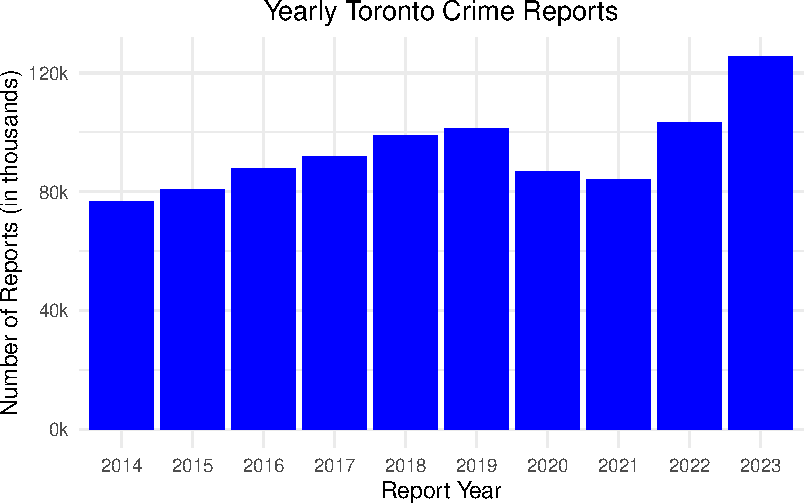
\includegraphics{paper_files/figure-pdf/fig-yearlycrimereport-1.pdf}

}

\caption{\label{fig-yearlycrimereport}Toronto Crime Reports per Year}

\end{figure}

Through this yearly crime type accumulation, we could oobviously
indicate that Theft has been the most commit crime in this decade. Even
during the COVID period, which has the least crime commit, theft still
kept the first place for all the commit crimes.
(Figure~\ref{fig-crimetype})

The majority of the reports in property crimes were from
(Figure~\ref{fig-theft}). Though there was a notable decline during the
onset of COVID-19 from approximately 50,000 in 2019 to approximately
39,000 in 2020, in 2023, there were over 68000 theft crime commit, which
was the highest record over the decade. This situation easily
reminiscent of the economic depression after COVID.

Besides theft, the commit of the other crimes were almost at the same
level, with Assault and Others each around 14000 issues per year and
15000 every year.Fraud has a rise trend these years, though with small
fluctuations, which starting from 4000 issues in 2014 till 12500 issues
in 2023. Fortunately, it is delight to figure that both robbery and
sexual violation almost had no variation, keeping around 2500 issues
every year. (Figure~\ref{fig-crime_type_notheft})

\begin{figure}

{\centering 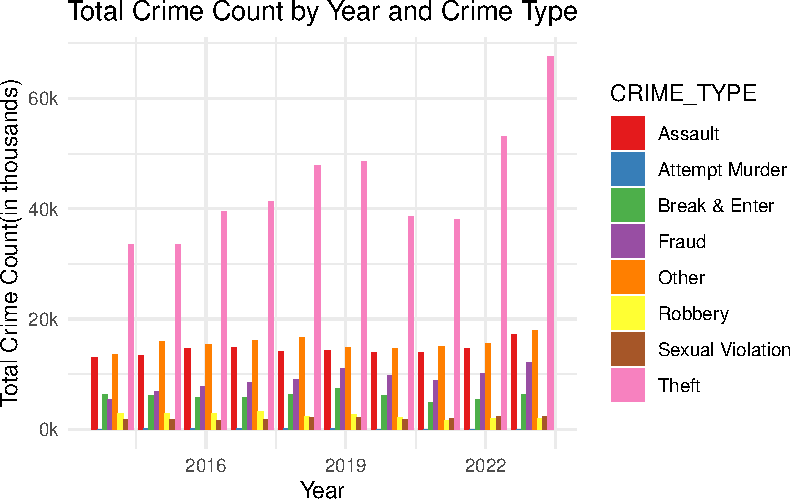
\includegraphics{paper_files/figure-pdf/fig-crimetype-1.pdf}

}

\caption{\label{fig-crimetype}Crime type commit in decades}

\end{figure}

\begin{figure}

{\centering 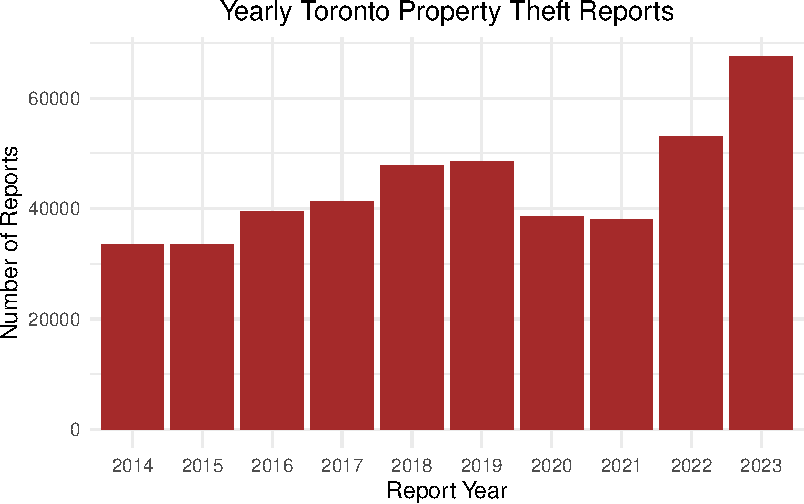
\includegraphics{paper_files/figure-pdf/fig-theft-1.pdf}

}

\caption{\label{fig-theft}Propert Theft Reports per Year in Toronto}

\end{figure}

\begin{figure}

{\centering 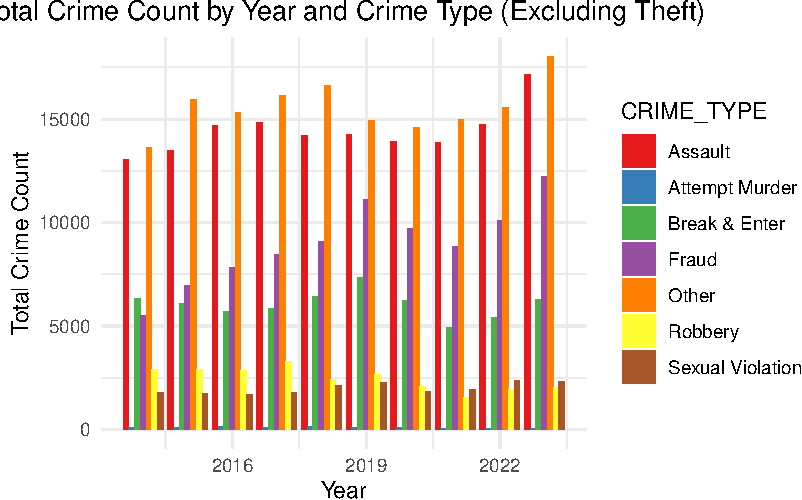
\includegraphics{paper_files/figure-pdf/fig-crime_type_notheft-1.pdf}

}

\caption{\label{fig-crime_type_notheft}Total Crime Count by Year and
Crime Type (Excluding Theft)}

\end{figure}

Despite the growth of property crime in 2023, the property crime commit
during and after COVID (2020-2023) was much more less than 2014-2019. In
order to check how much difference does each district has between these
two time period, Crime Against Property was listed out for the plot
below. Y- axis shows the percentage of difference of 2014- 2019 period
COVID Period divide 2014-2019 (Pre-COVID). We could observe that across
the 16 divisions in Toronto, Division 52 showed the most significant
change in 'Crimes Against Property'' during and after COVID-19, followed
by Division 41 and Division 43. This indicates that after COVID,
Division 52, 41 and 43 has made the most significant change in becoming
one of the most safety divisions among all the 16 divisions. On
contract, with only around 5\% difference, Division 13 shows almost no
difference this decade. (Figure~\ref{fig-divisioncrimechange}).

\begin{figure}

{\centering 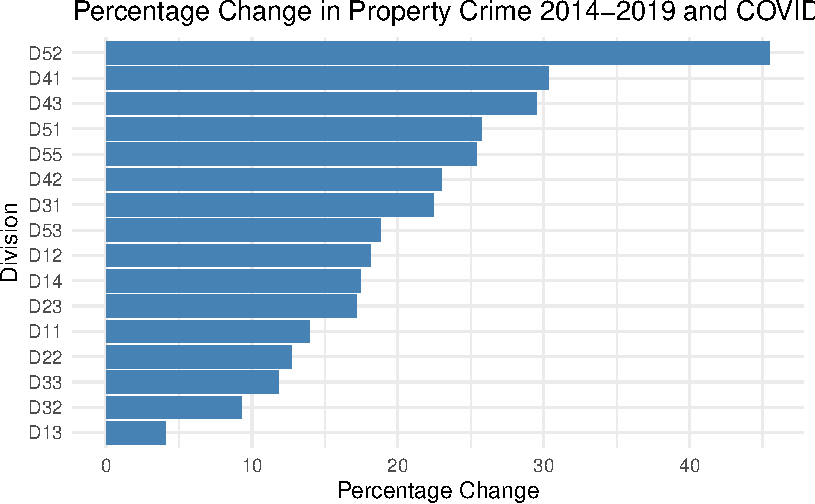
\includegraphics{paper_files/figure-pdf/fig-divisioncrimechange-1.pdf}

}

\caption{\label{fig-divisioncrimechange}Crime change in different
districts}

\end{figure}

\hypertarget{discussion}{%
\section{Discussion}\label{discussion}}

\hypertarget{total-trend-of-the-decade}{%
\subsection{Total trend of the decade}\label{total-trend-of-the-decade}}

The total crime trend in Toronto from 2014 to 2024 illustrates a complex
landscape of crime dynamics influenced by various social, economic, and
environmental factors.

Initially, the data shows a steady increase in total reported crimes,
reaching a peak in 2019. This escalation can be attributed to a growing
urban population, increased visibility of crime reporting, and possibly
rising economic disparities. The upward trend reflected the broader
challenges cities face, including issues related to housing, social
services, and community safety.

However, the onset of the COVID-19 pandemic in 2020 brought an
unexpected shift. During the early months of the pandemic, total crime
rates saw a decline, as lockdowns and restrictions limited movement and
increased police presence. This temporary drop indicated that certain
crimes were directly linked to the vibrancy of urban life---less
movement meant fewer opportunities for crimes like theft and burglary.

In 2021, as society began to adjust to pandemic-related restrictions,
the crime rate began to stabilize, but the data shows a gradual increase
again in subsequent years. By 2022 and 2023, crime rates surged to
unprecedented levels, surpassing pre-pandemic figures. This resurgence
can be linked to several factors, including the economic fallout from
the pandemic, rising unemployment, and social unrest.

Additionally, the increase in property crimes and thefts reflects the
broader economic struggles faced by many individuals during this period.
Communities that had been severely affected by the pandemic experienced
heightened vulnerability, leading to increased crime rates.

Overall, the total crime trend from 2014 to 2024 in Toronto reveals not
only the immediate impacts of the COVID-19 pandemic but also longer-term
socio-economic challenges. This trend underscores the importance of
understanding the underlying factors driving crime, the need for
responsive law enforcement strategies, and the role of community support
systems in fostering public safety and resilience in urban environments.

\hypertarget{covid-influence}{%
\subsection{COVID Influence}\label{covid-influence}}

The COVID-19 pandemic significantly impacted various facets of life,
including crime patterns in Toronto. Initially, as lockdowns and
restrictions were enforced, many types of crime, especially property
crimes, saw a decrease due to heightened police presence and the reduced
movement of people. However, as the city adapted to new norms and
restrictions began to ease, a troubling trend emerged: theft and
property crimes surged.

Though the data we could clearly find that from 2022 onward, the data
shows a marked increase in theft-related incidents. This rise can be
attributed to several factors. Firstly, economic challenges stemming
from the pandemic led to job losses and financial instability for many
residents, which may have driven some individuals toward crime as a
means of survival. Secondly, with more people spending time at home and
businesses adjusting to new operating procedures, opportunities for
theft became more apparent, particularly in residential areas.

By 2023, thefts had escalated significantly compared to pre-pandemic
levels, raising concerns among residents and law enforcement. This spike
in theft illustrates how the pandemic not only altered daily life but
also reshaped the landscape of crime in Toronto, revealing the complex
interplay between societal challenges and criminal behavior.

\hypertarget{district-safety}{%
\subsection{District Safety}\label{district-safety}}

With the data showing that some district has made numerous change in
strengthen the safety, Toronto is actively endeavouring to ensure the
safety of its inhabitants. As crime rates fluctuate across
neighborhoods, Toronto Polices are enthusiastic in decreasing the
overall crime rate these year. For instance, areas that have implemented
neighborhood watch programs and increased police visibility report
enhanced public safety and community cohesion.

Looking to the future, Toronto's commitment to safety encompasses not
only addressing immediate concerns but also fostering long-term
strategies. Urban planning initiatives that prioritize green spaces,
improved lighting, and accessible public resources can significantly
enhance crime prevention efforts. Furthermore, ongoing collaboration
between law enforcement, community organizations, and residents is
essential to adapt to evolving challenges. By emphasizing sustainable
safety measures and empowering community participation, Toronto aims to
create a safer environment that promotes resilience and well-being for
all its residents. This holistic approach will not only mitigate crime
but also cultivate a sense of community belonging and trust among
citizens.

\newpage

\hypertarget{references}{%
\section*{References}\label{references}}
\addcontentsline{toc}{section}{References}

\hypertarget{refs}{}
\begin{CSLReferences}{1}{0}
\leavevmode\vadjust pre{\hypertarget{ref-citeR}{}}%
R Core Team. 2023. \emph{R: A Language and Environment for Statistical
Computing}. Vienna, Austria: R Foundation for Statistical Computing.
\url{https://www.R-project.org/}.

\end{CSLReferences}



\end{document}
